\chapter{Pasivní detektory používané k monitorování kosmického záření}\label{sec:detektory_detektory}
Pasivní detektory nepotřebují napájení, jsou dobře skladné (malé rozměry, malá hmotnost) a bezpečné, což je činí vhodnými měřícími prostředky ve vesmíru. Mezi jejich hlavní zápory patří, že nedodávají data v reálném čase a že pro vyhodnocení musí být zpravidla dopraveny na Zem do příslušné laboratoře~\cite{benton}.

K monitorování kosmického záření se používají hlavně termoluminiscenční detektory (TLD) a detektory stop v pevné fázi (TED, nuclear track etched detectors/solid state nuclear track detectors). V menší míře se využívají i detektory založené na opticky stimulované luminiscenci (OSLD), bublinkové detektory \ldots V této kapitole rozebereme TLD a TED.

Výstupem z TLD je dávka, která se absorbovala v detektoru za celý čas měření, avšak nezjistí se kvalita záření (většinou). Oproti tomu pomocí TED je navíc možné změřit $\mathit{LET}$ spektrum v rozsahu, který je rozebrán dále v textu; $\mathit{LET}$ je lineární přenos energie. Kombinací dat z TLD a z TED lze určit celkový dávkový ekvivalent~\cite{benton}.
\section{Termoluminiscenční detektory}\label{sec:detektory_TLD}
Termoluminiscence je jev vyskytující se u některých pevných látek. Jeho podstata spočívá v tom, že je-li látka ozářena, pak při zahřívání vyzařuje světlo, jehož množství je přímo úměrné energii, která byla při ozáření v látce deponována. Zjednodušeně lze jev vysvětlit následovně: ionizující záření při interakci s látkou mimo jiné vytrhává elektrony z valenčního pásu, čímž vznikají iontové páry (záporný elektron a kladná díra) a vytržené elektrony přecházejí do vodivostního pásu. Část vytržených elektronů anihiluje s děrami (což uvolňuje tepelnou energii), avšak některé z nich se zachytí na tzv. elektronových pastech (nehomogenity v látce atp.). Aby se elektron z pasti dostal, tak mu musí být dodána energie k překonání vazby, což se děje při zahřívání látky. Uvolněný elektron následně
anihiluje s dírou, přičemž energie je vyzářena ve formě elektromagnetického záření (přibližně ve viditelném spektru) nebo je předána tzv. luminiscenčnímu centru, které energii taktéž přemění na světlo. Luminiscenční centra mohou být tvořena stopovými příměsemi prvků (např. Mn, Dy, Tm, Cu, C, \ldots). Světelný signál je zesílen fotonásobičem a poté vyhodnocen. 

Dodání energie pro vytržení elektronu z pasti nemusí být prováděno jen zahříváním látky, ale třeba i jejím osvícením. Tento jev je nazýván optická luminiscence a jsou na něm založeny OSLD.

Pro vyhodnocení TL signálu je důležitým pojmem vyhřívací křivka TLD, což je závislost světelného toku (respektive elektrického signálu z fotonásobiče) na teplotě. Odezva TLD se určí právě z této křivky (např. jako plocha pod křivkou, plocha pod píkem, výška píku~\cite{dosis}) a na základě kalibrace ve známém zdroji lze určit absorbovanou dávku.

TLD měří spolehlivě částice s $\mathit{LET}$ nižším než cca 10 keV/$\mu$m (tato hodnota se liší pro různé materiály), pro vyšší hodnoty $\mathit{LET}$ se účinnost TLD snižuje~\cite{passDetectors}. Pro lepší popis tohoto jevu se zavádí veličina relativní odezva detektoru $\mathit{RR}$ (relative response)
\begin{equation}
  \mathit{RR}=\frac{\left(TL_{\text{odezva}}/D_{\text{tkáň}}\right)_Y}{\left(TL_{\text{odezva}}/D_{\text{tkáň}}\right)_{\gamma}}\,,
  \label{eq:detektory_TLD_RR}
\end{equation}
kde $(TL_{\text{odezva}})_Y$, resp. $(TL_{\text{odezva}})_{\gamma}$ je odezva TLD po ozáření dávkou $(D_{\text{tkáň}})_Y$, resp. $(D_{\text{tkáň}})_{\gamma}$, přičemž tyto dávky jsou si číselně rovny. Jinak řečeno $\mathit{RR}$ je definována jako poměr odezev po ozáření stejnou dávkou v tkáni způsobenou částicemi $Y$ a referenčním zářením $\gamma$~\cite{TLD_RR}. 

Na vývoj $\RR$ se podíváme u dvou TLD používaných Oddělením dozimetrie záření ÚJF AV ČR (v dalším textu je používána anglická zkratka NPI, Nuclear Physics Institute). Jedná se o detektory Al$_2$O$_3$:C a CaSO$_4$:Dy. Tyto detektory byly, resp. jsou používány v experimentech DOSIS a DOSIS3D. V obr. \ref{fig:detektory_TLD_RR} jsou hodnoty relativní odezvy (relativní vůči $^{60}$Co) těchto detektorů pro částice s různým $\LET$ získané při experimentálním ozařování~\cite{dataTLD_RR}. Lze pozorovat, že s rostoucím $\LET$ relativní odezva u obou detektorů klesá, u Al$_2$O$_3$:C mnohem rychleji než u CaSO$_4$:Dy. Pro zpřesnění měření v polích částic s různým $\LET$ je potřeba provést korekci TL odezev, jinak dochází k podhodnocení dávky; více informací v~\cite{TLD_RR}.
\begin{figure}[H]
  \centering
  % GNUPLOT: LaTeX picture with Postscript
\begingroup
  \makeatletter
  \providecommand\color[2][]{%
    \GenericError{(gnuplot) \space\space\space\@spaces}{%
      Package color not loaded in conjunction with
      terminal option `colourtext'%
    }{See the gnuplot documentation for explanation.%
    }{Either use 'blacktext' in gnuplot or load the package
      color.sty in LaTeX.}%
    \renewcommand\color[2][]{}%
  }%
  \providecommand\includegraphics[2][]{%
    \GenericError{(gnuplot) \space\space\space\@spaces}{%
      Package graphicx or graphics not loaded%
    }{See the gnuplot documentation for explanation.%
    }{The gnuplot epslatex terminal needs graphicx.sty or graphics.sty.}%
    \renewcommand\includegraphics[2][]{}%
  }%
  \providecommand\rotatebox[2]{#2}%
  \@ifundefined{ifGPcolor}{%
    \newif\ifGPcolor
    \GPcolortrue
  }{}%
  \@ifundefined{ifGPblacktext}{%
    \newif\ifGPblacktext
    \GPblacktexttrue
  }{}%
  % define a \g@addto@macro without @ in the name:
  \let\gplgaddtomacro\g@addto@macro
  % define empty templates for all commands taking text:
  \gdef\gplbacktext{}%
  \gdef\gplfronttext{}%
  \makeatother
  \ifGPblacktext
    % no textcolor at all
    \def\colorrgb#1{}%
    \def\colorgray#1{}%
  \else
    % gray or color?
    \ifGPcolor
      \def\colorrgb#1{\color[rgb]{#1}}%
      \def\colorgray#1{\color[gray]{#1}}%
      \expandafter\def\csname LTw\endcsname{\color{white}}%
      \expandafter\def\csname LTb\endcsname{\color{black}}%
      \expandafter\def\csname LTa\endcsname{\color{black}}%
      \expandafter\def\csname LT0\endcsname{\color[rgb]{1,0,0}}%
      \expandafter\def\csname LT1\endcsname{\color[rgb]{0,1,0}}%
      \expandafter\def\csname LT2\endcsname{\color[rgb]{0,0,1}}%
      \expandafter\def\csname LT3\endcsname{\color[rgb]{1,0,1}}%
      \expandafter\def\csname LT4\endcsname{\color[rgb]{0,1,1}}%
      \expandafter\def\csname LT5\endcsname{\color[rgb]{1,1,0}}%
      \expandafter\def\csname LT6\endcsname{\color[rgb]{0,0,0}}%
      \expandafter\def\csname LT7\endcsname{\color[rgb]{1,0.3,0}}%
      \expandafter\def\csname LT8\endcsname{\color[rgb]{0.5,0.5,0.5}}%
    \else
      % gray
      \def\colorrgb#1{\color{black}}%
      \def\colorgray#1{\color[gray]{#1}}%
      \expandafter\def\csname LTw\endcsname{\color{white}}%
      \expandafter\def\csname LTb\endcsname{\color{black}}%
      \expandafter\def\csname LTa\endcsname{\color{black}}%
      \expandafter\def\csname LT0\endcsname{\color{black}}%
      \expandafter\def\csname LT1\endcsname{\color{black}}%
      \expandafter\def\csname LT2\endcsname{\color{black}}%
      \expandafter\def\csname LT3\endcsname{\color{black}}%
      \expandafter\def\csname LT4\endcsname{\color{black}}%
      \expandafter\def\csname LT5\endcsname{\color{black}}%
      \expandafter\def\csname LT6\endcsname{\color{black}}%
      \expandafter\def\csname LT7\endcsname{\color{black}}%
      \expandafter\def\csname LT8\endcsname{\color{black}}%
    \fi
  \fi
    \setlength{\unitlength}{0.0500bp}%
    \ifx\gptboxheight\undefined%
      \newlength{\gptboxheight}%
      \newlength{\gptboxwidth}%
      \newsavebox{\gptboxtext}%
    \fi%
    \setlength{\fboxrule}{0.5pt}%
    \setlength{\fboxsep}{1pt}%
\begin{picture}(7936.00,5102.00)%
    \gplgaddtomacro\gplbacktext{%
      \csname LTb\endcsname%
      \put(814,704){\makebox(0,0)[r]{\strut{}0.2}}%
      \csname LTb\endcsname%
      \put(814,1163){\makebox(0,0)[r]{\strut{}0.3}}%
      \csname LTb\endcsname%
      \put(814,1622){\makebox(0,0)[r]{\strut{}0.4}}%
      \csname LTb\endcsname%
      \put(814,2082){\makebox(0,0)[r]{\strut{}0.5}}%
      \csname LTb\endcsname%
      \put(814,2541){\makebox(0,0)[r]{\strut{}0.6}}%
      \csname LTb\endcsname%
      \put(814,3000){\makebox(0,0)[r]{\strut{}0.7}}%
      \csname LTb\endcsname%
      \put(814,3459){\makebox(0,0)[r]{\strut{}0.8}}%
      \csname LTb\endcsname%
      \put(814,3919){\makebox(0,0)[r]{\strut{}0.9}}%
      \csname LTb\endcsname%
      \put(814,4378){\makebox(0,0)[r]{\strut{}1.0}}%
      \csname LTb\endcsname%
      \put(814,4837){\makebox(0,0)[r]{\strut{}1.1}}%
      \csname LTb\endcsname%
      \put(946,484){\makebox(0,0){\strut{}$1$}}%
      \csname LTb\endcsname%
      \put(3144,484){\makebox(0,0){\strut{}$10$}}%
      \csname LTb\endcsname%
      \put(5341,484){\makebox(0,0){\strut{}$100$}}%
      \csname LTb\endcsname%
      \put(7539,484){\makebox(0,0){\strut{}$1000$}}%
    }%
    \gplgaddtomacro\gplfronttext{%
      \csname LTb\endcsname%
      \put(176,2770){\rotatebox{-270}{\makebox(0,0){\strut{}$\mathit{RR}$ [-]}}}%
      \put(4242,154){\makebox(0,0){\strut{}$\mathit{LET}$ [keV/$\mu$m]}}%
      \csname LTb\endcsname%
      \put(6552,4538){\makebox(0,0)[r]{\strut{}Al$_2$O$_3$:C}}%
      \csname LTb\endcsname%
      \put(6552,4066){\makebox(0,0)[r]{\strut{}CaSO$_4$:Dy}}%
    }%
    \gplbacktext
    \put(0,0){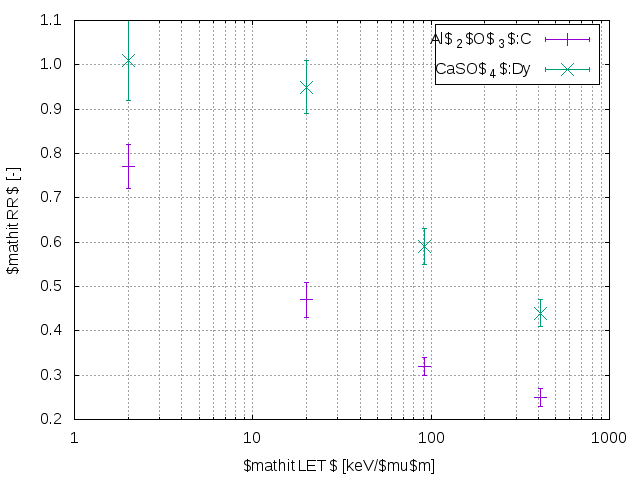
\includegraphics{TLD_RR}}%
    \gplfronttext
  \end{picture}%
\endgroup

  \caption{Relativní odezva dvou detektorů používaných NPI pro částice s různým $\LET$. Data pocházejí z~\cite{dataTLD_RR}.}
  \label{fig:detektory_TLD_RR}
\end{figure}
\section{Detektory stop v pevné fázi}
V některých pevných látkách vznikají při ozáření stabilní mikropoškození, tzv. latentní stopy, které mohou být vhodným způsobem zvětšeny. Následně lze zvětšené stopy spočítat např. pomocí mikroskopu, přičemž počet stop je úměrný počtu částic, které s materiálem interagovaly. Používají-li se tyto látky jako detektory ionizujícího záření, pak je nazýváme detektory stop v pevné fázi (TED). Z velikosti stop lze určit $\LET$ a $D$ (dávka) odpovídající částice a tím i dávkový ekvivalent $H$. Mezi materiály s touto schopností patří různá skla, minerální krystaly, plasty, nedávno byla tato vlastnost objevena i u některých kovů, intermetalických sloučenin a supravodivých oxidů; tento jev byl poprvé pozorován v roce 1958 u krystalů LiF \cite{objevTED}. Jako TED
se používají hlavně plasty, skla a minerální krystaly.

TED jsou schopné měřit pouze částice s $\LET$ vyšším než je určitá prahová hodnota, jež je různá pro odlišné materiály. Pro plasty, které jsou nejcitlivější, se pohybuje kolem 10 keV/$\mu$m~\cite{ambrozova_dvaExperimenty}. Rozsah měřitelných $\LET$ je omezený i shora, tato hodnota také zavisí na materiálu.  

Latentní stopy jsou nejčastěji zvětšovány chemickým leptáním. Tato metoda vychází z faktu, že poškozené části materiálu se leptají rychleji než nepoškozené. Někdy se používá dvoustupňové (per partes) leptání, které má tu výhodu, že po první fázi jsou zřetelné stopy vytvořené částicemi s krátkým dosahem a s velkým $\LET$ ($> 300$ keV/$\mu$m), které by při jednostupňovém dlouhém leptání byly odstraněny, a po druhé fázi naopak lze identifikovat stopy vytvořené částicemi s malým $\LET$ (až do detekčního prahu), čímž se významně zvýší rozsah detekovatelných částic \cite{cesky}. 

Tvorba latentních stop není doposud plně pochopena. U anorganických materiálů se jej snaží vysvětlit např. mechanismus popsaný v \cite{spikeModel}. U organických materiálů je proces tvorby stop rozdělen do tří fází: fáze fyzikální, fáze fyzikální-chemická a fáze chemická. Při první fázi ztrácí částice v materiálu energii (excitacemi a ionizacemi elektronů z obalu terčíků, vyražením terčíku z polymerové vazby, brzdným záření v případě velké rychlosti částice). Při druhé fázi dochází k interakcím částic vzniklých v první fázi, které vyúsťují ke vzniku latentních stop; latentní stopa se skládá z jádra o průměru cca 10 nm a vnější oblasti o průměru odpovídající dosahu delta elektronů, viz obr. \ref{fig:detektory_latentTrack}. Poslední fáze představuje leptání, při němž jsou stopy zafixovány
a zvětšeny.~\cite{thesisKPBrabcova} 
\begin{figure}[h]
  \centering
  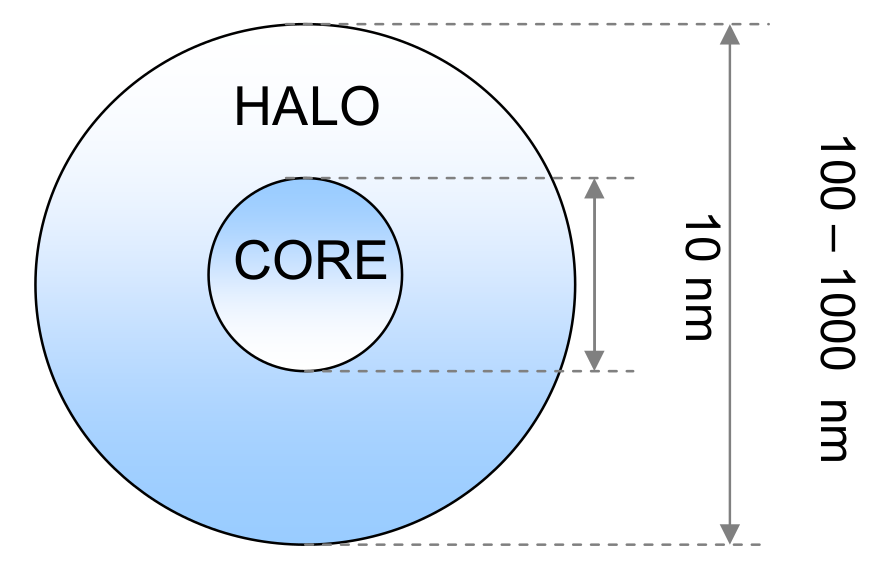
\includegraphics[width=0.38\textwidth]{detektory_latentTrack.png}
  \caption{Latentní stopa v organickém materiálu se skládá z jádra (CORE) a z obalu (HALO). \cite{thesisKPBrabcova}}
  \label{fig:detektory_latentTrack}
\end{figure}

Řada vnějších parametrů hraje roli při tvorbě stop v plastech. Například absence kyslíku v okolním prostředí a vyšší teploty způsobují, že vznikající stopy jsou menší a detektor má sníženou citlivost~\cite{ambrozova_dvaExperimenty}.

Nejpoužívanějším TED materiálem je poly allyl diglykolkarbonát, který bývá často také nazýván CR-39 (zkratka původního výrobního jména Columbia Resin \#39 \cite{CR39_wiki}). Jako detektor stop v pevné fázi se začal používat ke konci 70. let 20. století \cite{thesisKPBrabcova}; ve vesmírné dozimetrii byl poprvé použit při prvním letu amerických raketoplánů Space Shuttle v roce 1981 \cite{benton}. Původní CR-39 byl schopen detekovat částice s $\LET$ vyšším než cca 5 keV/$\mu$m \cite{benton}. V současné době je vyráběn pod různými jmény a s různými úpravami; také do něho bývají přidány další přísady, které mají zlepšit jeho vlastnosti. Některé úpravy ovlivňují i účinnost detekce částic s menším $\LET$, což jinými slovy znamená zvýšení detekčního prahu.~\cite{thesisKPBrabcova} 
%psát o ageing a fading???
%citovani v tomto oddile zvlastni
\subsection{Vyhodnocování}
Důležitou charakteristikou leptání je tzv. poměr leptacích rychlostí, definovaný vztahem
\begin{equation}
  V=\frac{V_S}{V_M}\,,
  \label{eq:pomerLepRychlostiDEF}
\end{equation}
kde $V_M$ je rychlost leptání nepoškozeného materiálu a $V_S$ rychlost leptání poškozeného materiálu, tj. stopy. Z provedených experimentů se ukazuje, že $V_S$ je konstantní u stop vytvořených částicemi s velkým dosahem, avšak např. u stop vytvořených sekundárními částicemi konstantní není~\cite{ssntd}. My jej však budeme obecně brát konstantní, protože tímto způsobem je vyhodnocována většina TED. Z poměru leptacích rychlostí lze z experimentálně zjištěného vztahu určit $\LET$ částice, jež stopu vytvořila. Nejprve si tedy ukážeme, jak zjistit $V$.

Po leptání detektoru jsou stopy analyzovány. K tomu se např. používá mikroskop s kamerou, která nasnímá povrch detektoru. Zvětšení je takové, aby stopy byly snadno rozpoznatelné; stopy jsou znázorněny jako tmavé elipsoidní objekty, viz obr. \ref{fig:detektory_stopy}. Snímky mohou být dále zpracovány v příslušném programu; osy všech elips/stop (hlavní osa $a$, vedlejší osa $b$) jsou výstupem programu. 
%Ve vyhodnocovacím softwaru jsou pak stopy brány jako elipsy, výstupem softwaru jsou velikosti hlavní a vedlejší osy. 
Poměr leptacích rychlostí může být určen z hodnot $a,b$ pro každou stopu ze vztahu
\begin{equation}
  V=\frac{\sqrt{\left( 1-B^2 \right)^2}+4A^2}{1-B^2}\,,
  \label{eq:pomerLepRychlosti}
\end{equation}
kde
\begin{align*}
  A&=\frac{a}{2V_Mt}\,,\\
  B&=\frac{b}{2V_Mt}
\end{align*}
a $t$ je doba, po kterou se leptalo, tj. $d=V_Mt$ je tloušťka odleptané vrstvy nepoškozeného materiálu; vztahy byly převzaty z~\cite{ssntd}. Existuje více metod zjištění $d$. Je možné přímo měřit hodnoty tlouštěk materiálu před a po leptání a poté je odečíst. Mnohem přesnější je např. metoda štěpných fragmentů; tato a další metody jsou popsány v~\cite{thesisKPBrabcova}.    
%\begin{equation}
  %h=V_bt,
  %\label{eq:thicknessOfMaterial}
%\end{equation}
\begin{figure}[ht]
  \centering
  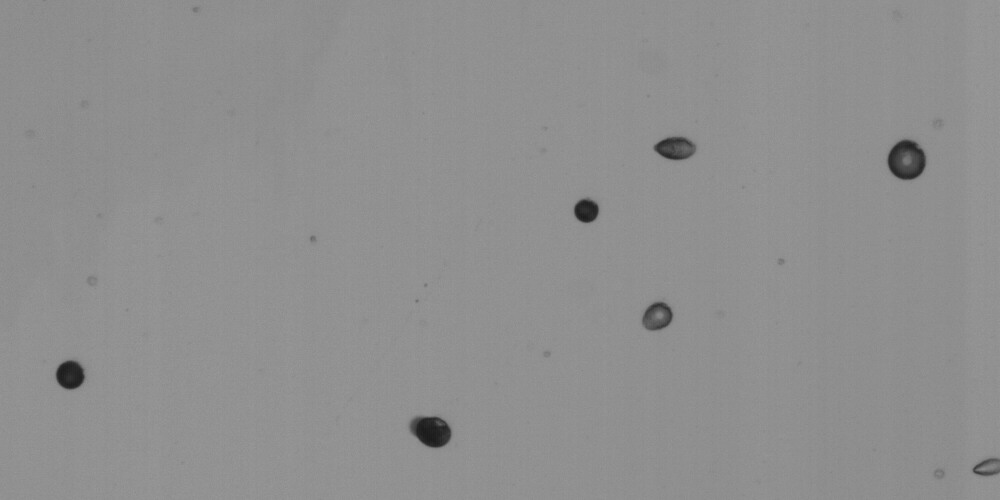
\includegraphics[width=0.7\textwidth]{praktickaCast_stopyOK.jpg}
  \caption{Část plochy detektoru zaznamenaná mikroskopem, stopy jsou tmavé elipsoidní objekty.}
  \label{fig:detektory_stopy}
\end{figure}

Kalibrační křivka, neboli vztah mezi $V$ a $\LET$, je určena experimentálním ozařováním příslušného TED. Pro proklad naměřených dat lze použít nejrůznější funkce, příkladem je polynom třetího stupně, který má výhodu jednoduchosti. Je důležité poznamenat, že od určitých hodnot $\LET$ nejsou k dispozici kalibrační body, a proto jsou za touto hranicí určené hodnoty $\LET$ zatížené velikou nepřesností.

Existuje minimální úhel dopadu částice na detektor, při němž je stopa stále ještě po leptání zřetelná, tj. není leptáním odstraněna. Tento úhel se nazývá kritický úhel a je definován vztahem $\theta_k=1/V$. Počet detekovaných částic na plochu $N$ je třeba opravit na částice, které dopadly pod menším úhlem než $\theta_k$; za předpokladu izotropního rozložení dopadajících částic (což lze ve vesmíru brát jako splněné) to je možné provést vynásobením koeficientem 
\begin{equation}
  k_{\theta}=\frac{V^2}{V^2-1},
  \label{eq:kritickyUhel}
\end{equation}
tedy $N^{\text{kor}}=N\cdot k_{\theta}$. 

Celková absorbovaná dávka $D$ a dávkový ekvivalent $H$ můžeme určit ze vztahů 
\begin{align}
  D&=\int\text{konst}\cdot\LET\frac{dN^{\text{kor}}}{d\LET}d\LET\,,\label{eq:Davka}\\
  H&=\int\text{konst}\cdot\LET\cdot Q(\LET)\frac{dN^{\text{kor}}}{d\LET}d\LET\,,\label{eq:EkvDavka}
\end{align}
kde $\frac{dN^{\text{kor}}}{d\LET}$ je opravený počet částic na plochu mající $\LET$ v intervalu $d\LET$; $Q$ je jakostní faktor určený podle tab. \ref{tab:detektory_Q} a $\text{konst}=1,602\cdot 10^{-6}$ je převodní konstanta. Vztah byl převzat z~\cite{thesisKPBrabcova}.

\begin{table}[H]
  \centering
  \caption{Hodnoty jakostního faktoru $Q$ v závislosti na $\LET$ (ICRP 60, 1991).}
  \label{tab:detektory_Q}
  \begin{tabular}{ll}
	\toprule
	$\LET$ [keV/$\mu$m]&$Q(\LET)$ \\
	\midrule
$<$10&1\\
$[10;100]$&$0,32\LET-2,2$\\
$>$100&300/$\sqrt{\LET}$\\
	\bottomrule
  \end{tabular}
\end{table}
\section{Kombinace dat z TLD a TED}
Citlivosti TLD a TED se celkem dobře doplňují, a tak lze tyto dva druhy pasivních detektorů využít ke změření celkové absorbované dávky a celkového dávkového ekvivalentu. Ze známosti relativní odezvy TL detektoru a z $\LET$ spektra získaným z dat změřených detektorem stop lze odečíst příspěvek částic s vysokým $\LET$ (tedy takových, pro které je $\RR<1$) od dávky změřené TLD. Zbylá dávka z TLD pocházející od částic s malým $\LET$ se pak pričte k dávce určené TED, která pochází od částic s vyšším $\LET$. Tímto způsobem je získána celková absorbovaná dávka. Celkový dávkový ekvivalent se stanoví součtem upravené dávky TLD (pro nízké $\LET$ platí $Q=1$, viz tab. \ref{tab:detektory_Q}) a dávkovým ekvivalentem TED.~\cite{dataTLD_RR}


%vyhodnocování OSLD probíhá pomocí referenčního zdroje (ten vztah asi nepsat) (dosis, s. 7); OSLD detektory se tato práce nezabývá, takže spíš ne

%napsat z ceho jsou vyrobene (nebo spis co presne jsou) TLD pouzivane NPI (prasek, krystal atd.)

%HSP1000 -> jediny v Evrope!!!!!!!!!!! (viz stranky ODZ UJF AVCR) -> to uz je v praktickaCast


%Nevýhodou pasivních detektorů je skutečnost, že po každém měření musely být dopraveny zpět na Zem do příslušné laboratoře a teprve tam byly vyhodnoceny; avšak oproti aktivním detektorům nemusejí být napájeny proudem, což je v prostředí ISS velmi praktické. %toto asi až to další kapitoly o detektorech

